\chapter{Mòduls i llibreries}
Els mòduls ens permeten empaquetar les nostres funcions i organitzar-les modularment. Quan hem vist la llibreria {\tt math} el que hem realitzat és una importació del mòdul. Quan utilitzem {\tt import} fem que sempre hagem d'incloure el nombre del mòdul abans d'accedir als mètodes o atributs. Al incloure-les és un bon patró fer-ho de la manera següent.

\begin{blockcode}
import math
\end{blockcode}

També podem crear un alias o abreviació per a treballar de manera més ràpida amb el módul utilitzant l'opció {\tt as}. Així doncs amb la següent forma accediríem als mètodes amb {\tt mt.} 

\begin{blockcode}
import math as mt
mt.sin(2)
\end{blockcode}

És millor utilitzar {\tt import} que {\tt from modul import} degut a que la segona manera ens importarà funcions que quan tinguem projectes grans no sabrem d'on provenen i de vegades podem tenir col·lisions de noms, que és quan dues funcions o variables tenen el mateix nom i una sobreescriu l'altre.

\begin{blockcode}
from math import *
\end{blockcode}

Com hem vist amb el mòdul {\tt math} nosaltres podem importar el mòdul i després accedir a les funcions membre i als atributs mitjançant el punt '.'. Nosaltres també podem crear el nostre mòdul de manera senzilla. Podem desar en un arxiu un conjunt de funcions i una crida a aquestes per a que s'executin. Guardem les següents funcions dins d'un fitxer anomenat {\tt funcions.py}.

\begin{blockcode}
def quadrat(x):
    return x**2
def cub(x):
    return x**3
\end{blockcode}
Un cop creat el fitxer nosaltres podem importar-lo emprant el nom del fitxer. Sempre buscarà en els fitxers dintre del nostre directori de treball. 
\begin{blockcode}
>>> import funcions
>>> funcions.cub(3)
27
\end{blockcode}
\section{NumPy}
NumPy és una llibreria de Python per a treballar amb arrays multidimensionals i especialment amb arrays grans. Implementa funcions d'àlgebra i està implementada a baix nivell per a un processament ràpid. Per a poder treballar amb NumPy haurem d'importar el mòdul.
\begin{blockcode}
>>> import numpy
>>> import numpy as np 
>>> from numpy import * 
\end{blockcode}
Per a la sessió assumirem que importem el mòdul com {\tt np} que degut al seu us intensiu és més breu i més còmode d'usar.

\subsection{Declaració d'arrays}
Amb NumPy declarem de la següent forma un array:

\begin{tip}[caption=Iicialització d'array amb NumPy]
>>> arr = np.array([[1,2],[3,4]])
>>> arr
array([[1, 2],
       [3, 4]])
\end{tip}


Per defecte el tipus de les dades serà detectat automàticament per Numpy. Podem comprobar el tipus de dades emprant l'atribut membre {\tt dtype}.


\begin{blockcode}
>>> arr.dtype
dtype('int64')
\end{blockcode}

Els tipus de dades estan homogeneïtzats. Així doncs si declarem totes les variables com a enters i una d'elles com a real, llavors tots els nombres seran reals.

\begin{blockcode}
>>> arr = np.array([[1,2],[3,4.3]])
>>> arr.dtype
dtype('float64')
>>> arr
array([[ 1.,  2.],
       [ 3.,  4.3]])
\end{blockcode}
Al contrari que en les llistes de Python tots els tipus han de ser del mateix tipus. També podem especificar el tipus {\tt int}, tant com a segon paràmetre, com utilitzant la declaració implícita {\tt dtype=int}.
\begin{blockcode}
>>> arr = np.array([[1,2.9],[3,4.3]], dtype=int)
>>> arr.dtype
dtype('int64')
>>> arr
array([[1, 2],
       [3, 4]])
\end{blockcode}
També podem especificar el tipus {\tt complex}.
\begin{blockcode}
>>> arr = np.array([[1,2.9],[3,4.3]], dtype=complex)
>>> arr.dtype
dtype('complex128')
>>> arr
array([[ 1.0+0.j,  2.9+0.j],
       [ 3.0+0.j,  4.3+0.j]])
\end{blockcode}
A continuació llistem els diversos tipus de dades que podem utilitzar a NumPy. Depenent de les necessitats del nostre programa utilitzarem un o altre.
\begin{itemize}
\item bool
\item complex64
\item complex128
\item complex256
\item float32
\item float64
\item float128
\item int8
\item int16
\item int32
\item int64
\item uint8
\item uint16
\item uint32
\item uint64
\end{itemize}
La funció {\tt zeros()} ens permet inicialitzar una matriu. També li podem especificar el tipus de dades amb el que volem treballar.

\begin{tip}[caption=Inicialització amb funcio zeros()]
>>> z = np.zeros((2,2), dtype=int)
>>> z
array([[0, 0],
       [0, 0]])
>>> z.dtype
dtype('int64')
>>> z = np.zeros((2,2), dtype=complex)
>>> z
array([[ 0.+0.j,  0.+0.j],
       [ 0.+0.j,  0.+0.j]])
>>> z = np.zeros((2,2), dtype=float)
>>> z
array([[ 0.,  0.],
       [ 0.,  0.]])
\end{tip}


També tenim la funció anàloga {\tt ones}.

\begin{tip}[caption=Inicialització amb funcio ones()]
>>> o = np.ones((3,3), np.float128)
>>> o
array([[ 1.,  1.,  1.],
       [ 1.,  1.,  1.],
       [ 1.,  1.,  1.]])
\end{tip}


També es pot donar el cas en que tenim una matriu M i volem crear una matriu amb les mateixes dimensions que M i inicialitzar-la amb zeros o uns. Per això tenim les funcions {\tt ones\_like} i {\tt zeros\_like}, que ens copien les dimensions d'una matriu donada.


\begin{tip}[caption=Zeros like i ones like]
>>> m = np.array([[1,2],[3,4],[5,6]])
>>> m
array([[1, 2],
       [3, 4],
       [5, 6]])
>>> z = np.zeros_like(m)
>>> z
array([[0, 0],
       [0, 0],
       [0, 0]])
>>> o = np.ones_like(m)
>>> o
array([[1, 1],
       [1, 1],
       [1, 1]])
\end{tip}

Per a crear llistes tal i com fins ara fèiem emprant la funció {\tt range} podem utilitzar la funció  de NumPy {\tt arange}


\begin{blockcode}
>>> np.arange(20,-20,-2)
array([ 20,  18,  16,  14,  12,  10,   8,   6,   4,   2,   
0,  -2,  -4,  -6,  -8, -10, -12, -14, -16, -18])
\end{blockcode}
Degut a problemes de la representació de les dades, casos en els que utilitzem nombres reals pot succeir que es propaguin errors de representació i que el nombre d'elements retornat no sigui previsible. Per això utilitzem la funció {\tt linspace} on primer especifiquem
\begin{blockcode}
>>> np.linspace(-2,2,6)
array([-2. , -1.2, -0.4,  0.4,  1.2,  2. ])
\end{blockcode}
També podem emprar la funció {\tt linspace} per a crear seqüències de nombres complexos.
\begin{blockcode}
>>> np.linspace(-3+4j,2+7j,9)
array([-3.000+4.j , -2.375+4.375j, -1.750+4.75j, -1.125+5.125j,
       -0.500+5.5j,  0.125+5.875j,  0.750+6.25j,  1.375+6.625j,
        2.000+7.j   ])
\end{blockcode}
Podem crear una llista d'elements emprant la funció {\tt linspace} i després convertir-la en una matriu emprant la funció {\tt reshape}. Aquesta funció també redimensiona amb altres matrius.

\begin{tip}[caption=Combinació de linspace() i reshape()]
>>> arr = np.linspace(-2,2,6)
>>> arr.reshape((2,3))
array([[-2. , -1.2, -0.4],
       [ 0.4,  1.2,  2. ]])
\end{tip}


Si volem construir una matriu identitat cridem la funció la funció {\tt identity}. Així doncs, per a crear la següent matriu
\[ \left( \begin{array}{ccc}
1 & 0 & 0 \\
0 & 1 & 0 \\
0 & 0 & 1 \end{array} \right)\] 
Necessitem saber les dimensions de la matriu, que al ser la matriu identitat una matriu quadrada només és un paràmetre. En el cas previ 3.
\begin{blockcode}
>>> np.identity(3)
array([[ 1.,  0.,  0.],
       [ 0.,  1.,  0.],
       [ 0.,  0.,  1.]])
\end{blockcode}
\subsection{Accés a les dades}
Podem accedir a les dades tal i com accedíem a llistes bidimensionals, o amb els índex separats per comes a dins del claudators.
\begin{blockcode}
>>> a = np.array([[1, 2, 3], [4, 5, 6]], float)
>>> a
array([[ 1.,  2.,  3.],
       [ 4.,  5.,  6.]])
>>> a[0,2]
3.0
>>> a[0][2]
3.0
\end{blockcode}
Hem de tindre en compte un concepte molt important en la còpia de les arrays, i es que al realitzar una assignació entre variables de numpy no estem copiant, sinó que estem creant una altre referència al mateix objecte.
\begin{blockcode}
>>> x = np.zeros((3,3))
>>> x
array([[ 0.,  0.,  0.],
       [ 0.,  0.,  0.],
       [ 0.,  0.,  0.]])
>>> y = x
>>> y[1,1] = -1
>>> x
array([[ 0.,  0.,  0.],
       [ 0., -1.,  0.],
       [ 0.,  0.,  0.]])
>>> y
array([[ 0.,  0.,  0.],
       [ 0., -1.,  0.],
       [ 0.,  0.,  0.]])
\end{blockcode}
Per evitar-ho el que fem és us de la funció {\tt copy}


\begin{tip}[caption=Còpia per valor mitjançant la funció copy()]
>>> x = np.zeros((3,3))
>>> x
array([[ 0.,  0.,  0.],
       [ 0.,  0.,  0.],
       [ 0.,  0.,  0.]])
>>> y = x.copy()
>>> y[1,1] = -1
>>> x
array([[ 0.,  0.,  0.],
       [ 0.,  0.,  0.],
       [ 0.,  0.,  0.]])
>>> y
array([[ 0.,  0.,  0.],
       [ 0., -1.,  0.],
       [ 0.,  0.,  0.]])
\end{tip}


Podem comprovar si un element es troba a dins d'una llista mitjançant la funció {\tt in}
\begin{blockcode}
>>> 4 in a
True
>>> -4 in a
False
\end{blockcode}
Trobar elements dins d'un array. Fem servir la funció {\tt where}
\begin{blockcode}
>>> x = numpy.array([1,0,2,0,3,0,4,5,6,7,8])
>>> numpy.where(x == 0)[0]
array([1, 3, 5])
\end{blockcode}
\subsection{Operacions amb matrius}
Per la suma de tots els elements de la matriu utilitzem la funció utilitzem la funció {\tt sum} i per a realitzar el producte la funció {\tt prod}
\begin{blockcode}
>>> o = np.ones((3,4), complex)
>>> o.sum()
(12+0j)
>>> o.prod()
(1+0j)
\end{blockcode}
Aquestes funcions estan implementades a baix nivell amb C per a la seva rapidesa, i són molt més ràpides que si nosaltres declarem un bucle en Python que realitzi aquesta mateixa tasca.
També tenim funcions per a trobar el mínim i el màxim a dins de la funció amb les funcions {\tt min} i {\tt max}, i per a saber els seus índex dintre de l'array emprarem les funcions {\tt argmin} i {\tt argmax}.
\begin{blockcode}
>>> m
array([[1, 2],
       [3, 4],
       [5, 6]])
>>> m.min()
1
>>> m.max()
6
>>> m.argmin()
0
>>> m.argmax()
5
\end{blockcode}
NumPy també inclou funcions estadístiques per a realitzar càlculs amb els arrays. Tenim per a la mitja la funció {\tt mean} per a la variança la funció {\tt var} i per a la desviació estàndard la funció {\tt std}
\begin{blockcode}
>>> m
array([[1, 2],
       [3, 4],
       [5, 6]])
>>> m.mean()3.5
>>> m.var()
2.9166666666666665
>>> m.std()
1.707825127659933
\end{blockcode}
La funció {\tt diagonal} ens retorna els valors de la diagonal de la matriu.
\begin{blockcode}
>>> i = np.identity(3)
>>> i.diagonal()
array([ 1.,  1.,  1.])
\end{blockcode}
Podem concatenar arrays utilitzan la funció {\tt hstack}
\begin{blockcode}
np.hstack(v1, v2)
\end{blockcode}
Per a multiplicar matrius utilitzem la funció {\tt dot} i per a redimensionar una matriu utilitzem {\tt reshape}
\begin{blockcode}
>>> x = np.arange(9).reshape((3,3))
>>> y = np.arange(3)
>>> np.dot(x,y)
array([ 5, 14, 23])
\end{blockcode}
\section{MatplotLib}
Matplotlib proporciona una llibreria que permet graficar conjunts de valors amb diferents formes de representació. És utilitzada en l'àmbit científic i busca ser una alternativa a altres paquets com Matlab. Matplotlib també te la forma acceptada com estàndard \emph{de facto} d'importar el mòdul al igual que Numpy. En aquest cas es crida {\tt plt}. El mòdul que cridem és en veritat un submòdul que s'anomena {\tt pyplot}.
\begin{blockcode}
import matplotlib.pyplot as plt
\end{blockcode}
Per a tots els exemples que mostrarem assumirem que el mòdul NumPy i matplotlib estan importats com {\tt np} i {\tt plt}
\subsection{Aproximació a Matplotlib}
Per fer a generar els gràfics sempre haurem de cridar a una funció específica per a cada gràfic. El gràfic de línies s'utilitza mitjançant la funció {\tt plot()} com es mostra a l'exemple 01. La funció {\tt show} s'encarrega d'obrir una nova finestra que 


\begin{tip}[caption=Plot sencill]
>>> plt.plot([1,2,3,4,5])
>>> plt.show()
\end{tip}


\begin{figure}[!h]
    \begin{centering}
    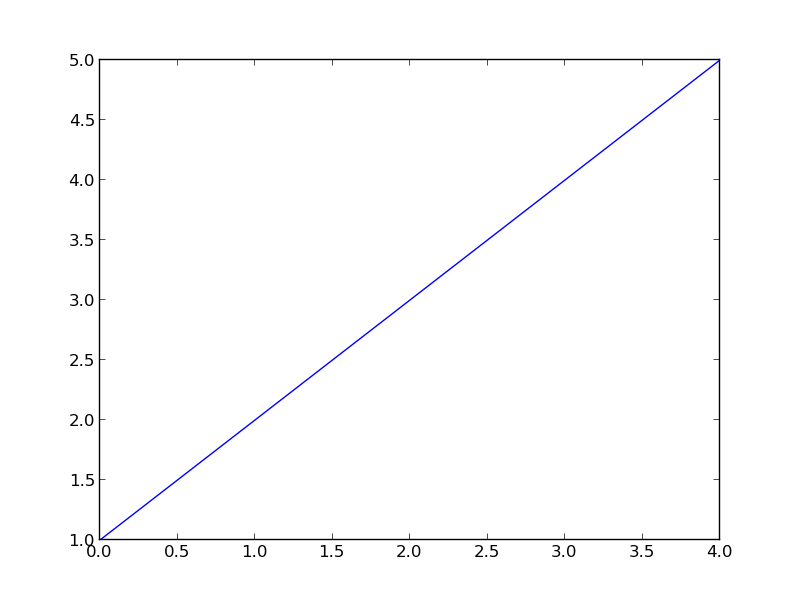
\includegraphics[width=0.35\textwidth]{img/ex01.png}
    \caption{exemple plot simple}
    \label{fig:figex01}
    \end{centering}
\end{figure}


No només podem utilitzar les llistes pròpies de Python, sinó que podem utilitzar funcions i arrays de Numpy per a mostrar-les tal i com es mostra a l'exemple 02.

\begin{tip}[caption=Sinusoidal amb matplotlib]
np.arange(0, 2*np.pi, 0.1);
y = np.sin(x)
plt.plot(x, y)
\end{tip}


\begin{figure}[!h]
    \begin{centering}
    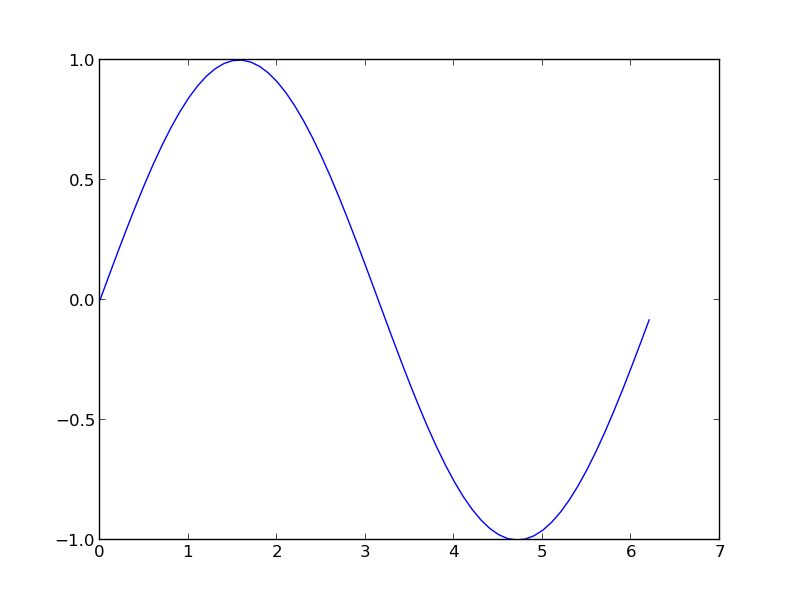
\includegraphics[width=0.35\textwidth]{img/ex02.png}
    \caption{exemple sinosoidal}
    \label{fig:figex02}
    \end{centering}
\end{figure}
Si no volem tindre que cridar la funció {\tt show()} cada cop que volem fer un {\tt plot}, llavors haurem d'activar el mode interactiu amb la funció {\tt ion()} (interactive on). Aquest mode és molt útil quan estem treballant amb una terminal i no volem cridar la funció {\tt show} cada cop que volem veure els resultats.
\begin{blockcode}
plt.ion()
\end{blockcode}
Podem apagar-lo amb la funció anàloga {tt iof}.
\begin{blockcode}
plt.ioff()
\end{blockcode}
Per a tots els exemples que mostrarem assumirem que el mode interactiu està desactivat. Podem comprovar l'estat d'aquest mode mitjançant la funció
\begin{blockcode}
plt.isinteractive()
\end{blockcode}
\subsection{Gràfics}
Abans hem vist la funció {\tt plot} per realitzar gràfiques simples. A continuació veurem diverses funcions de matplotlib per a mostrar diferents menes de gràfics.

\subsection{Scatter}
En el cas de plot nosaltres tenim una distribució que va avançant seqüencialment. Quan volem repartir punts aleatòriament per l'espai utilitzarem la funció {\tt scatter}. La funció rep dos paràmetres, l'eix de les x i de les Y

\begin{tip}[caption=Funcio scatter]
plt.scatter([2.5,2,3],[3,2,1])
plt.show()
\end{tip}

\begin{figure}[!h]
    \begin{centering}
    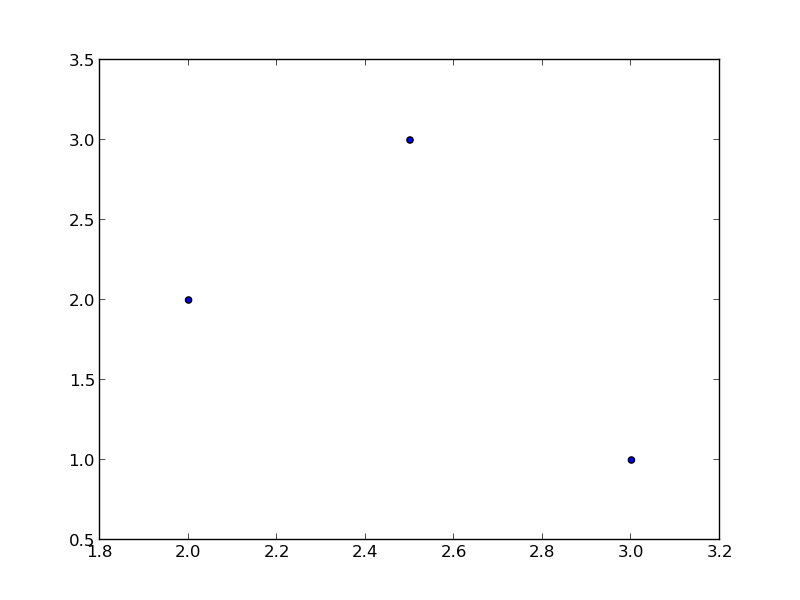
\includegraphics[width=0.3\textwidth]{img/ex03.png}
    \caption{exemple scatter}
    \label{fig:figex03}
    \end{centering}
\end{figure}

\subsection{Gràfics de barres}
Pels gràfics de barres es crida a la funció {\tt bar} i es passen els dos eixos (X,Y) com a paràmetre de la funció. També existeix una altre funció per barres que es específica per a divisions de colors o reparticions de valors tal i com histogrames que s'anomena {\tt hist}.

\begin{tip}[caption=Gràfic de barres]
plt.bar([1,2,3],[4,9,2])
\end{tip}


\begin{figure}[!h]
    \begin{centering}
    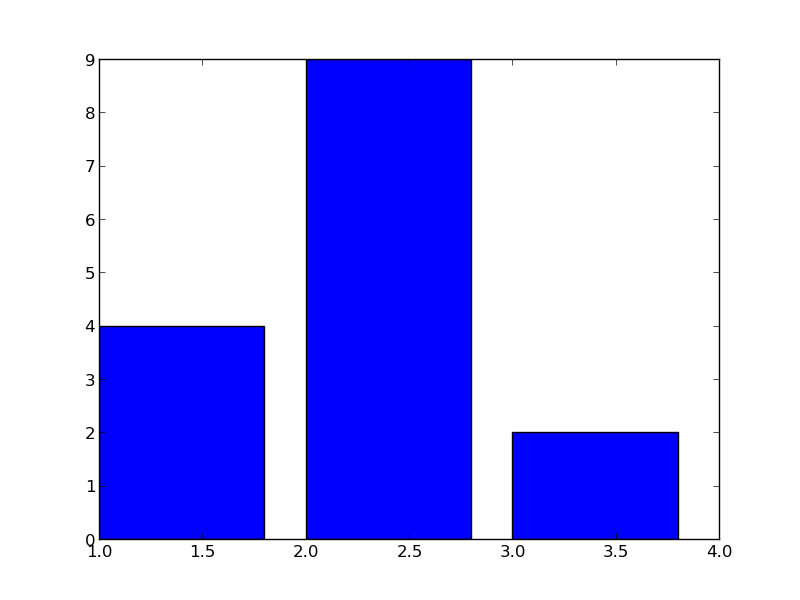
\includegraphics[width=0.3\textwidth]{img/ex04.png}
    \caption{gràfic de barres}
    \label{fig:figex04}
    \end{centering}
\end{figure}
\subsection{Gràfics pastís}
Aquest gràfic ens sumarà tots els valors i cada part agafarà la part de l'angle que li correspongui.


\begin{tip}[caption=Gràfic pastís]
plt.pie([1,2,3,4,5,6])
\end{tip}


\begin{figure}[!h]
    \begin{centering}
    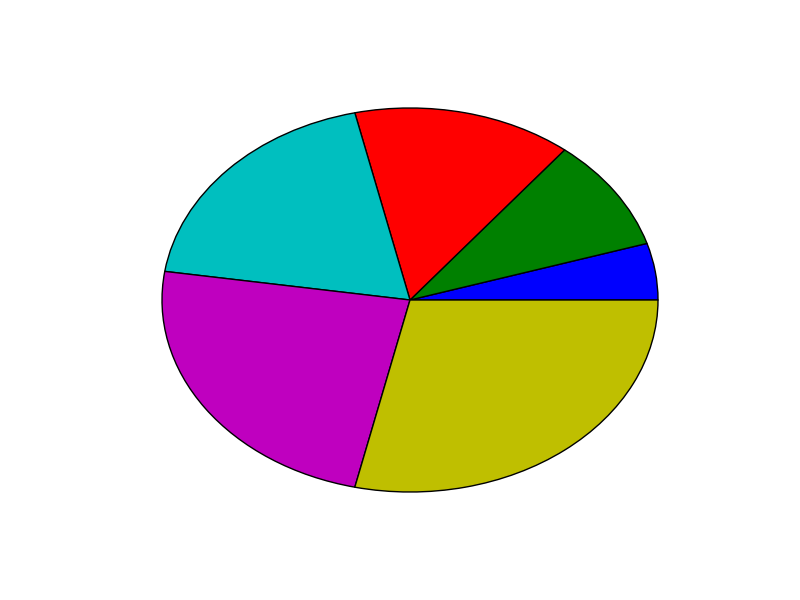
\includegraphics[width=0.35\textwidth]{img/ex05.png}
    \caption{gràfic pastís}
    \label{fig:figex05}
    \end{centering}
\end{figure}
\subsection{Gràfics  amb fletxes}
Aquests gràfics són utilitzats amb sistemes d'equacions diferencials o en valors de magnituds repartits per l'espai. Representen un vector amb una direcció i una llargària. Necessitem dues matrius, una amb l'eix de les X i una altre amb l'eix de les Y de les forces. Les fletxes van des de una coordenada (0,0) que està indicada en el punt de la matriu, al punt on està especificat el valor

\begin{figure}[!h]
    \begin{centering}
    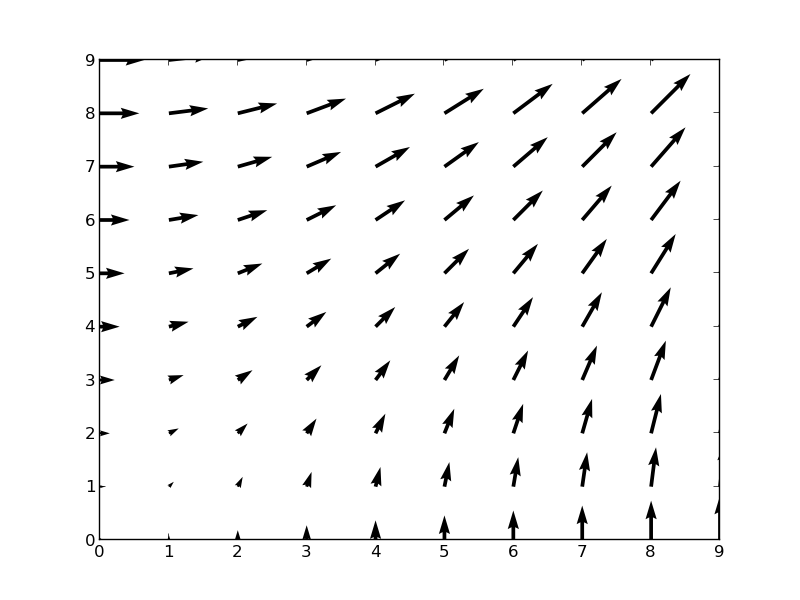
\includegraphics[width=0.3\textwidth]{img/ex06.png}
    \caption{exemple gràfic fletxes}
    \label{fig:figex06}
    \end{centering}
\end{figure}

\begin{tip}[caption=Gràfic fletxes]
X, Y = np.mgrid[0:10, 0:10]
plt.quiver(X, Y)
\end{tip}



\subsection{Guardar gràfics en arxiu}
Matplotlib permet guardar les gràfiques que hem realitzat dins d'una imatge. Per a poder guardar-la especifiquem la ruta del fitxer i el nom de la imatge

\begin{blockcode}
plt.savefig("exemple.png")
plt.savefig("exemple.pdf")
\end{blockcode}

\section{SciPy}
SciPy és una llibreria de Python que implementa un conjunt de funcions matemàtiques. A diferència que NumPy integra rutines numèriques com per exemple funcions per treballar amb vectors  o manipulació d'imatges. La seva finalitat es proveir a la comunitat científica d'un ventall de funcionalitats per a processament de dades. Normalment trobarem SciPy importat de la següent manera

\begin{blockcode}
import scipy as sp
\end{blockcode}
SciPy està organitzada en un conjunt de subpackets:
\begin{itemize}
\item \emph{cluster} Algoritmes de clustering
\item \emph{constants} Constants matemàtiques i físiques
\item \emph{fftpack} Rutines de la tranformada ràpida de Fourier
\item \emph{integrate} Integració i equacions diferencials ordinaries
\item \emph{interpolate} interpolació
\item \emph{io} Entrada i sortida
\item \emph{linalg} Àlgebra linial
\item \emph{ndimage} Processament d'imatges N-dimensionals
\item \emph{odr} Regressió de distància ortogonal.
\item \emph{optimize} Optimització i cerca d'arrels.
\item \emph{signal} Processament de senyal.
\item \emph{sparse} Matrius disperses.
\item \emph{spatial} Algoritmes i estructures de dades de problemes espaials.
\item \emph{special} Funcions especials.
\item \emph{stats} Funcions i distribucions estadístiques.
\item \emph{weave} Funcionalitats per integrar codi en C/C++ en el codi Python.
\end{itemize}
A la pàgina \href{http://docs.scipy.org/doc/scipy/reference/tutorial/}{Documentació de Scipy} podrem trobar les referències i descripcions de les funcionalitats.
\begin{blockcode}
>>> import scipy.optimize as optimize
>>> sp.info(optimize.fmin)
\end{blockcode}





\subsection{Exemple de SciPy}
Per a veure un exemple de les moltes funcionalitats que proveu SciPy implementarem un codi utilitzant el paquest {\tt linalg} i veurem com NumPy i SciPy es combinen.
\begin{blockcode}
>>> import numpy as np
>>> from scipy import linalg
>>> A = np.array([[1,2],[3,4]])
>>> A
array([[1, 2],
      [3, 4]])
>>> b = np.array([[5],[6]])
>>> b
array([[5],
      [6]])
>>> linalg.inv(A).dot(b) #slow
array([[-4. ],
      [ 4.5]]
>>> A.dot(linalg.inv(A).dot(b))-b #check
array([[  8.88178420e-16],
      [  2.66453526e-15]])
>>> np.linalg.solve(A,b) #fast
array([[-4. ],
      [ 4.5]])
>>> A.dot(np.linalg.solve(A,b))-b #check
array([[ 0.],
      [ 0.]])
\end{blockcode}

